\subsubsection{数据规范化修正}

首先将检测孕周 $w_i$ 数据小数化，并添加孕天数 $d_i$ 列，统计表格发现，男胎孕妇的 $209$ 号样本存在大写 \verb`W`，处理时需注意。女胎孕妇的 $187$ 号样本（孕妇代码 B044）存在 BMI 缺失，根据 $B M I_i=\frac{\text { 体重}_i (\mathrm{kg})}{\text { 身高 }_i (\mathrm{m})^2}$ 计算约为 $36.198$。另外，由该公式计算出的值（$BMI_{i.calc}$）与表格直接提供的值（$BMI_{i,table}$）中，孕女胎样本均满足：
$$ |\textit{BMI}_{i, \text{calc}} - \textit{BMI}_{i, \text{table}}| > 0.01 $$

而男胎孕妇有 $199$ 个样本不满足该条件，为保证统计严谨，本文将表格中男胎孕妇的 BMI 值进行修正。
同时，将表格中的``末次月经''与``检测日期''全部转化为\texttt{YYYY/MM/DD} 格式，便于后期分析。分析结果发现，男胎样本中有 $655$ 条数据呈现出``末次月经''与``检测日期''的差值不完全准确等于``孕天''，医院通常采用 B 超等临床手段可以校准孕期，故本文赋予相对误差 $\pm 15$（天），再检测发现仍有 $31$ 条数据存在较大差异。本文基于计算出的孕周进行填补。除此之外，本文还对某些数据作出如下处理与假设：
\begin{enumerate}[leftmargin=2em]
    \item 医学上通常以末次月经的第一天作为孕期的起点，对不含末次月经时间的 12 条数据基于检测孕周进行简单填补；
    \item 对怀孕次数 $\geq 3$ 的样本，为便于统计，均假设其怀孕次数为 $3$；
    \item 题干指出，X 染色体浓度数值可能出现负值，在此认为负值数据均为有效数据；
\end{enumerate}

\subsubsection{异常值处理}

正常的 GC 含量应在 $40\% \sim 60\%$ 之间，过高、过低或分布异常都意味着测序质量存在问题。经过统计并绘制小提琴图（图 \ref{fig:violin}），可发现大部分数据位于 $39\% \sim 41\%$ 之间。并且四分位点也位于该区间内，其余分布异常的离散点被本文视作测序质量存在问题。

\begin{figure} [H]
    \centering
    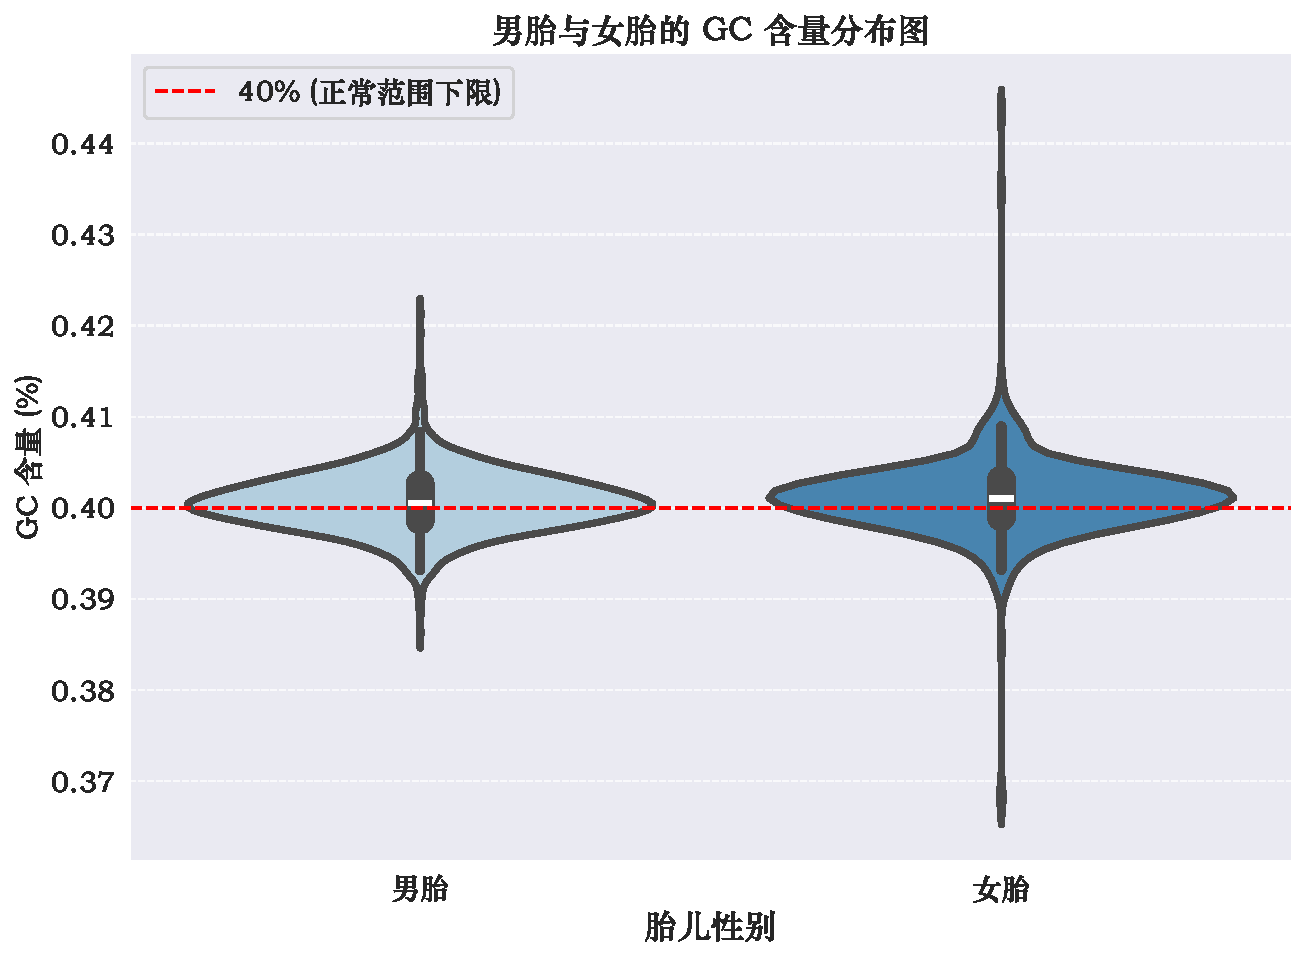
\includegraphics[width=0.8\textwidth]{chapters/数据预处理/images/数据清洗/GC值小提琴图.pdf}
    \caption{男胎与女胎的 GC 值小提琴图}
    \label{fig:violin}
\end{figure}

手动剔除分布不均匀的 $2$ 个 $GC < 0.39$ 的样本，以及 $2$ 个 $GC > 0.415$ 的样本，对于女胎样本，剔除分布不均匀的 $3$ 个 $GC < 0.39$ 的样本，以及 $2$ 个 $GC > 0.42$ 的样本。
